\chapter{Feature, scenari e storie}\label{ch-03}

\lecturemeta{Capitolo originale: 3 --- Features, Scenarios, and Stories \quad\textbullet\quad Antonio Brogi}{Appunti di Emiliano Sescu (github.com/Faxatos), cap. 3}

Il design di un prodotto software nasce di solito da uno di questi
fattori:

\begin{itemize}
\tightlist
\item
  l'ispirazione;
\item
  bisogni di aziende o consumatori che i prodotti esistenti non
  soddisfano;
\item
  insoddisfazione verso i prodotti esistenti;
\item
  cambiamenti tecnologici che rendono possibili nuovi tipi di prodotto.
\end{itemize}

In questo capitolo vediamo come arrivare alla specifica del prodotto che
vogliamo creare. Abbiamo già visto che discutere i requisiti con il
cliente è difficile, soprattutto per la differenza di linguaggio e
perché spesso il cliente non sa nemmeno quali funzionalità vuole.

Lo sviluppo product-based richiede meno documentazione di quello
project-based. In Agile i requisiti non li fissa il cliente e cambiano
spesso: per questo gli sviluppatori devono \textbf{individuare da soli
le feature} del prodotto, capendo chi sono i potenziali utenti e come
attirarli (con interviste, sondaggi, consultazioni informali, ecc.).

Per individuare le feature si usano rappresentazioni degli utenti
(\textbf{personas}) e descrizioni in linguaggio naturale
(\textbf{scenari} e \textbf{storie}).

\begin{figure}[H]
\centering
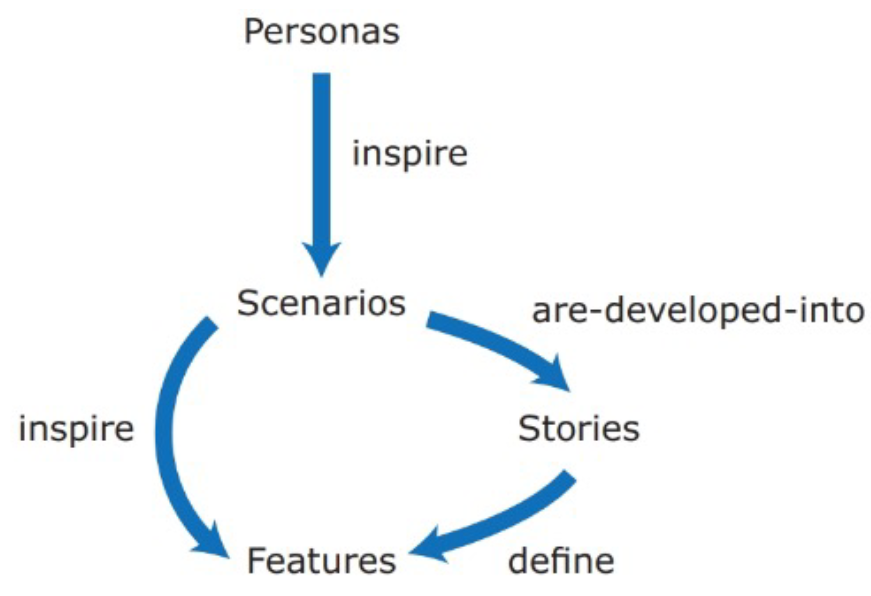
\includegraphics[width=0.49\linewidth,height=0.45\textheight,keepaspectratio]{images/03-feature_fig3-1_generazione-feature.png}
\caption{Il processo di generazione delle feature.}
\end{figure}

\section{Personas}\label{personas}

\begin{boxdefinition}{Persona}

Una \textbf{persona} è un utente tipo a cui si rivolge il prodotto,
descritto come se fosse una persona reale.

\end{boxdefinition}

Per progettare feature utili bisogna capire i potenziali utenti: il loro
background, le loro competenze e la loro esperienza influenzano
l'esperienza d'uso e l'interfaccia. Di solito bastano \textbf{poche
personas} (1-2, al massimo 5) per individuare le feature principali. Le
personas permettono agli sviluppatori di ``mettersi nei panni degli
utenti''.

Una persona si descrive con questi elementi:

\begin{itemize}
\tightlist
\item
  \textbf{Personalizzazione}: le si dà un nome e si descrive la sua
  situazione personale. A volte si usa anche una foto di repertorio:
  alcuni studi dicono che aiuta i team a usare meglio le personas.
\item
  \textbf{Lavoro} (\emph{job-related}): se il prodotto è per le aziende,
  si descrive il suo lavoro e (se serve) in cosa consiste. Per lavori
  noti a tutti, come l'insegnante, può non servire.
\item
  \textbf{Rilevanza}: se possibile, si spiega perché potrebbe
  interessarle il prodotto e cosa vorrebbe farci.
\item
  \textbf{Formazione}: si descrive il suo percorso di studi e il suo
  livello di competenze tecniche. È importante soprattutto per
  progettare l'interfaccia.
\end{itemize}

\begin{figure}[H]
\centering
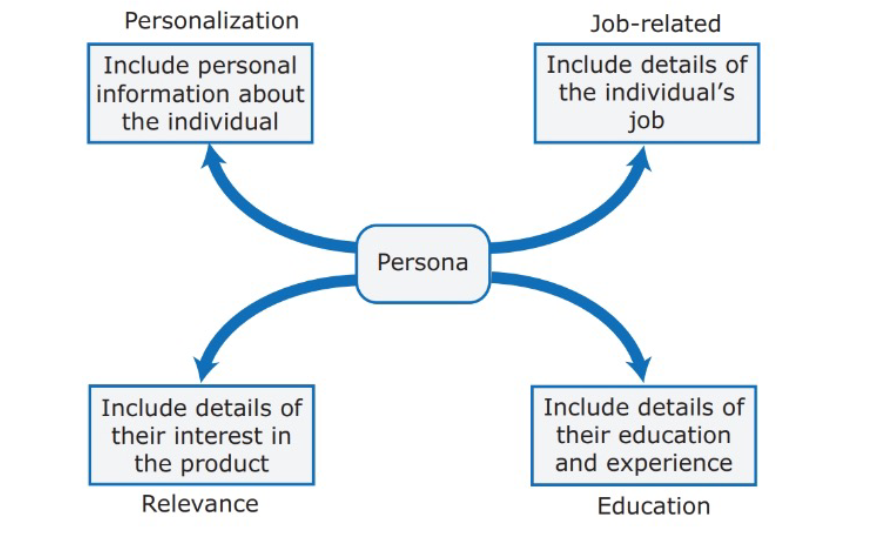
\includegraphics[width=0.80\linewidth,height=0.45\textheight,keepaspectratio]{images/03-feature_fig3-2_persona.png}
\caption{Gli elementi chiave di una persona.}
\end{figure}

L'uso della foto non è accettato da tutti: gli studi mostrano che la
foto ci condiziona con dei pregiudizi. Quando non è possibile studiare
gli utenti reali (ad esempio per prodotti del tutto nuovi) si creano
delle \textbf{proto-personas}, cioè personas immaginate.

\section{Scenari}\label{scenari}

Una volta create le personas, si passa agli scenari. Per scoprire le
feature del prodotto si descrivono scenari di interazione tra l'utente e
il prodotto.

\begin{boxdefinition}{Scenario}

Uno \textbf{scenario} è un racconto che descrive una situazione in cui
un utente usa le feature del prodotto per raggiungere un obiettivo
preciso.

\end{boxdefinition}

Uno scenario contiene questi elementi:

\begin{figure}[H]
\centering
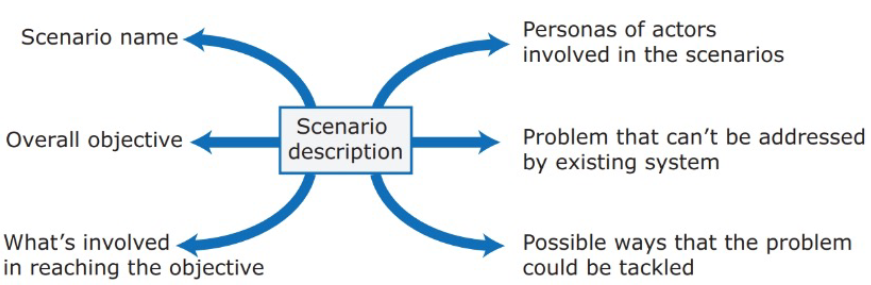
\includegraphics[width=0.80\linewidth,height=0.45\textheight,keepaspectratio]{images/03-feature_fig3-3_scenario.png}
\caption{Gli elementi chiave di uno scenario.}
\end{figure}

Gli scenari narrativi e di alto livello facilitano la comunicazione e
stimolano la creatività nel design. \textbf{Non sono però specifiche}:
mancano di dettagli e possono essere incompleti. Di solito servono più
scenari (es. 3-4) per ogni persona, che coprano le sue responsabilità
principali. Gli scenari si scrivono \textbf{dal punto di vista
dell'utente}.

\begin{boxtip}{Come si lavora sugli scenari}

Ogni membro del team scrive da solo alcuni scenari, poi li discute con
il resto del team e, se possibile, con gli utenti.

\end{boxtip}

\section{User Stories}\label{user-stories}

Gli scenari sono storie d'uso ad alto livello, mentre le \textbf{user
story} sono racconti più fini e seguono una struttura precisa:

\begin{boxdefinition}{User story}

\textbf{As a} \textless ruolo\textgreater{} \textbf{I want to}
\textless fare qualcosa\textgreater{} \textbf{so that} \textless motivo
/ valore\textgreater.

(Come \textless ruolo\textgreater{} voglio \textless fare
qualcosa\textgreater{} così da \textless motivo / valore\textgreater.)

\end{boxdefinition}

Le user story non fanno parte del manifesto Agile, ma aiutano a
rispettarne i principi:

\begin{itemize}
\tightlist
\item
  la priorità massima è soddisfare il cliente con consegne rapide e
  continue di software di valore;
\item
  il software funzionante è la misura principale del progresso;
\item
  la semplicità, l'arte di massimizzare il lavoro non fatto, è
  essenziale.
\end{itemize}

Le user story aiutano anche a \textbf{visualizzare l'avanzamento}: si
possono scrivere su post-it e attaccarle a una bacheca delle cose da
fare. Va ricordato però che:

\begin{itemize}
\tightlist
\item
  le storie che \textbf{non creano valore} per il cliente sono lavoro
  che non conta come progresso;
\item
  creare storie che \textbf{dipendono l'una dall'altra} può portare a
  situazioni di stallo (\emph{deadlock}).
\end{itemize}

Il product backlog di Scrum è spesso un insieme di user story. Le storie
lunghe (\textbf{epic}) vanno spezzate in storie più semplici. A ogni
storia si associa una \textbf{priorità} (e magari una stima dello
sforzo), e le storie si ordinano per priorità (\emph{requirements
triage}).

È possibile esprimere come user story tutte le funzionalità descritte in
uno scenario, ma gli scenari si leggono in modo più naturale: rendono le
storie più facili da capire, danno più contesto e sono più facili da
``vendere'' agli stakeholder.

\subsection{Dalle storie alle feature}\label{dalle-storie-alle-feature}

L'obiettivo finale delle user story è individuare le \textbf{feature}
che definiscono il prodotto. In linea di principio una feature dovrebbe
avere queste proprietà:

\begin{itemize}
\tightlist
\item
  \textbf{Indipendenza}: non deve dipendere da come sono implementate le
  altre feature, né dall'ordine in cui vengono attivate.
\item
  \textbf{Coerenza}: deve corrispondere a una sola funzionalità. Non
  deve fare più di una cosa e non deve mai avere effetti collaterali.
\item
  \textbf{Rilevanza}: deve riflettere il modo in cui gli utenti svolgono
  normalmente un compito. Niente funzionalità oscure che servono
  raramente.
\end{itemize}

Per progettare le feature servono quattro tipi di conoscenza:

\begin{figure}[H]
\centering
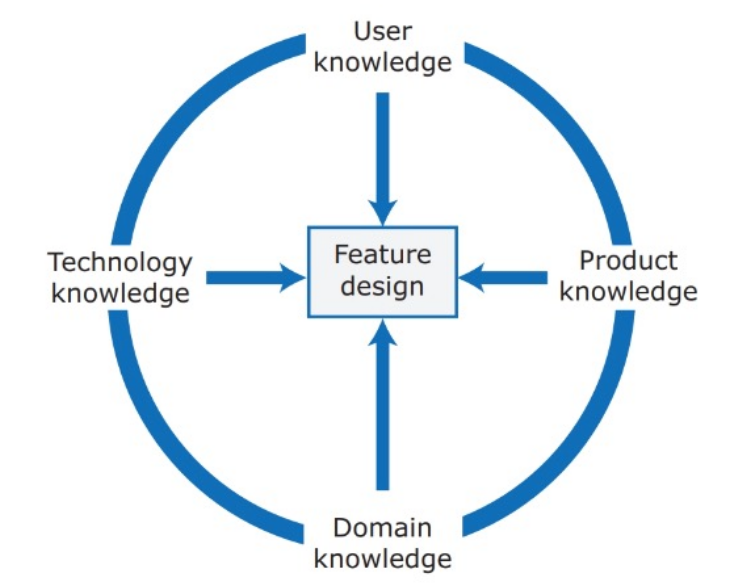
\includegraphics[width=0.60\linewidth,height=0.45\textheight,keepaspectratio]{images/03-feature_fig3-4_conoscenze.png}
\caption{Le conoscenze necessarie per il design delle feature.}
\end{figure}

\begin{itemize}
\tightlist
\item
  \textbf{Conoscenza degli utenti}: scenari e user story dicono al team
  cosa vogliono gli utenti e come potrebbero usare le feature.
\item
  \textbf{Conoscenza dei prodotti}: si può avere esperienza di prodotti
  esistenti, o studiarli durante lo sviluppo. A volte le feature devono
  replicare quelle dei prodotti esistenti, perché offrono funzionalità
  di base sempre necessarie.
\item
  \textbf{Conoscenza del dominio}: conoscere il settore in cui opera il
  prodotto (es. finanza, prenotazione di eventi) permette di pensare a
  modi nuovi per aiutare gli utenti a raggiungere i loro obiettivi.
\item
  \textbf{Conoscenza della tecnologia}: spesso i nuovi prodotti nascono
  per sfruttare tecnologie arrivate dopo i concorrenti. Chi conosce le
  tecnologie più recenti può progettare feature che le usano.
\end{itemize}

\subsection{Bilanciare i fattori e il feature
creep}\label{bilanciare-i-fattori-e-il-feature-creep}

Nel design delle feature bisogna trovare un equilibrio tra fattori
opposti.

\begin{figure}[H]
\centering
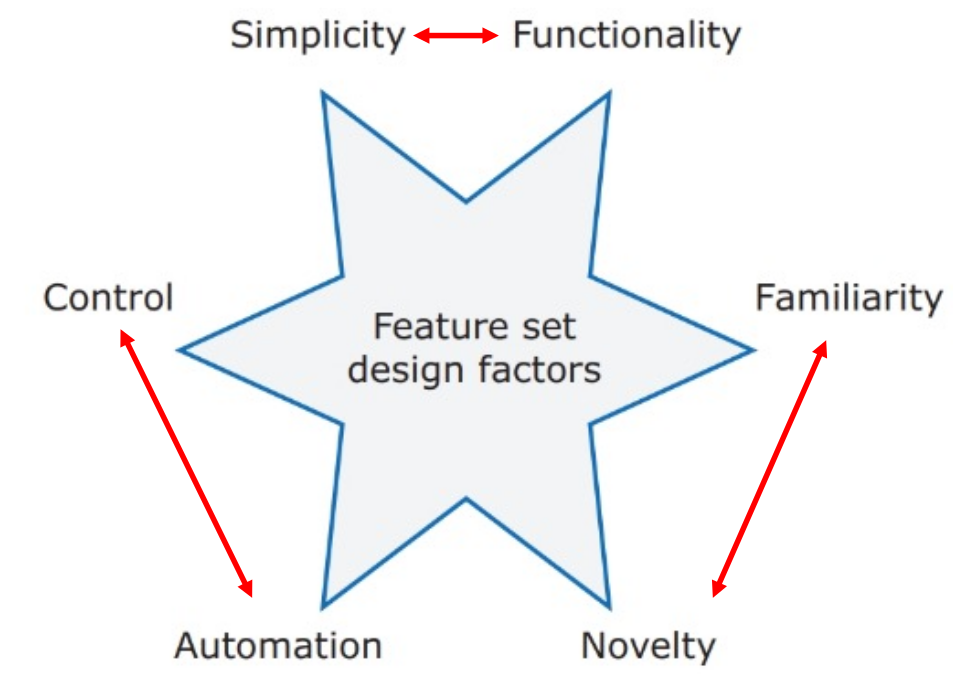
\includegraphics[width=0.60\linewidth,height=0.45\textheight,keepaspectratio]{images/03-feature_fig3-5_fattori-design.png}
\caption{I fattori nel design delle feature.}
\end{figure}

\begin{boxtip}{Le tre coppie in conflitto}

\begin{itemize}
\tightlist
\item
  \textbf{Semplicità vs funzionalità}: più funzioni aggiungi, più il
  prodotto diventa complicato da usare.
\item
  \textbf{Familiarità vs novità}: gli utenti vogliono ritrovare cose che
  conoscono, ma un prodotto nuovo deve anche offrire qualcosa di
  diverso.
\item
  \textbf{Automazione vs controllo}: automatizzare semplifica la vita,
  ma alcuni utenti vogliono decidere da soli cosa succede.
\end{itemize}

\end{boxtip}

Il numero di feature tende a crescere man mano che si immaginano nuovi
potenziali utenti: questo fenomeno si chiama \textbf{feature creep}. La
crescita è spinta dal marketing, che vuole accontentare tutte le
richieste degli utenti, aggiungere le feature dei concorrenti e
supportare sia utenti esperti sia principianti. Per evitare il feature
creep conviene porsi alcune domande su ogni feature, che aiutano a
capire quali sono inutili.

\begin{figure}[H]
\centering
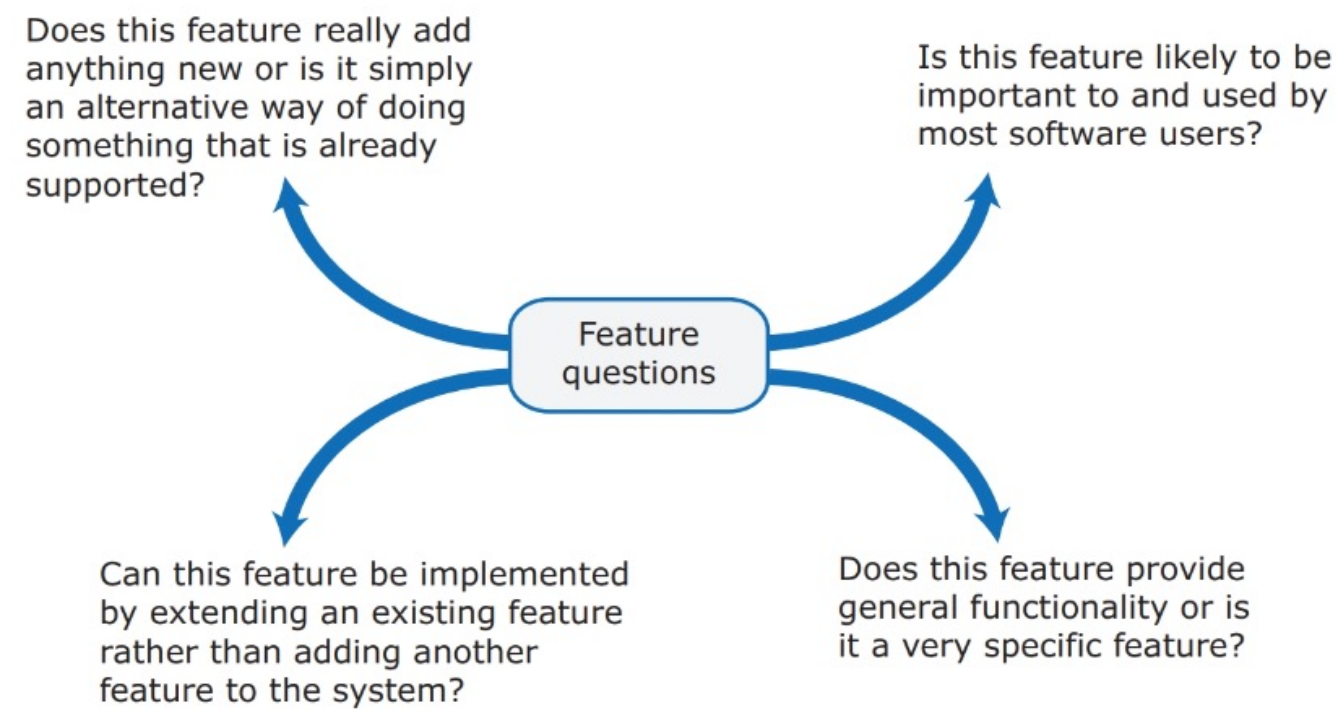
\includegraphics[width=0.90\linewidth,height=0.45\textheight,keepaspectratio]{images/03-feature_fig3-6_feature-questions.png}
\caption{Le domande sulle feature per evitare il feature creep.}
\end{figure}

\subsection{Derivare le feature}\label{derivare-le-feature}

Il team di sviluppo si riunisce per discutere scenari e storie e
ricavare la lista delle descrizioni delle feature. Per ogni feature si
individuano l'\textbf{input} e il modo in cui viene \textbf{attivata},
si descrive l'\textbf{azione} (come vengono elaborati i dati) e infine
si scrive l'\textbf{output} atteso.

\begin{figure}[H]
\centering
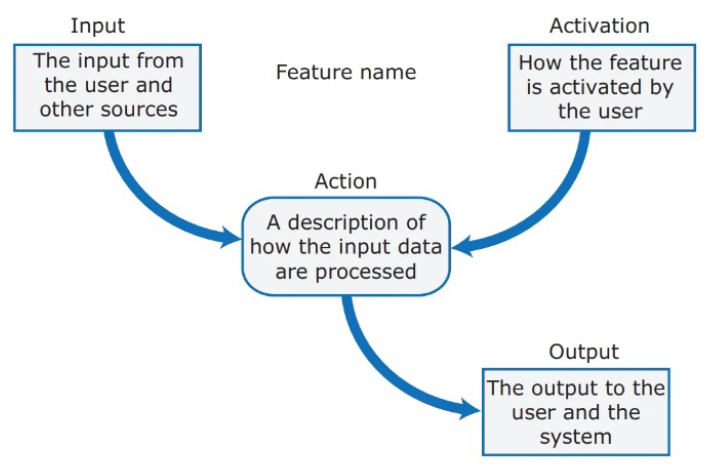
\includegraphics[width=0.80\linewidth,height=0.45\textheight,keepaspectratio]{images/03-feature_fig3-7_derivazione-feature.png}
\caption{Derivazione di una feature.}
\end{figure}
